%% == LaTeX PACKAGE tikz-3dplot-circleofsphere ================================
%%    Drawing circles of a sphere with tikz-3dplot
%% 
%% Matthias Wolff, BTU Cottbus-Sentenberg
%% July 26, 2018
%%
%% References:
%% [1] R. Niepraschk: The showexpl package. 2016. Online, retrieved July 23, 2018. 
%%     https://mirror.reismil.ch/CTAN/macros/latex/contrib/showexpl/doc/showexpl.pdf
%%     https://mirror.reismil.ch/CTAN/macros/latex/contrib/showexpl/doc/showexpl-test.pdf
%% [2] C. Heinz, B. Moses, and J. Hoffmann. The Listings Package. 2015. Online, retrieved July 23, 2018.
%%     http://mirror.hmc.edu/ctan/macros/latex/contrib/listings/listings.pdf
%%
\documentclass[a4paper]{article}
%
% Packages
\usepackage{amsmath}
\usepackage{amssymb}
\usepackage[dvipsnames]{xcolor}
\usepackage{xspace}
\usepackage{authblk}
\usepackage{url}
%\usepackage{bera}
\usepackage{afterpage}
\usepackage{longtable}
\usepackage{listings}
\usepackage{showexpl}
\usepackage{tikz}
\usepackage{tikz-3dplot}
\usepackage{tikz-3dplot-circleofsphere}
%
% Names
\newcommand{\tdplotCs}{\texttt{tikz-3dplot-circleofsphere}\xspace}
\newcommand{\tdplot}{\texttt{tikz-3dplot}\xspace}
%
% Custom commands
\newcommand\e{\mathrm{e}}
\renewcommand\i{\mathrm{i}}
\newcommand\atann{\mathop{\operatorname{arctan2}}}
\newcommand{\TT}[1]{\protect\scalebox{0.75}[1.04]{\texttt{#1}}}
\newcommand{\CORR}[1]{{\color{red!90!RoyalBlue}#1}}
\newcommand{\workOn}{\color{Salmon!80!black}}
\newcommand{\workOff}{\color{black}}
\newcommand{\TODO}[1]{%
  \fboxsep=1pt\fboxrule=1pt\fcolorbox{yellow}{white}{[\textbf{TODO:~}#1]}%
}
\newcommand{\CHECK}[1]{%
  \fboxsep=1pt\fboxrule=1pt\fcolorbox{yellow}{white}{#1}%
}
\newcommand\docCmd[2]{%
  \bigskip\noindent%
  \fboxsep=3pt
  \fcolorbox{black!5}{black!5}{\parbox{\linewidth}{%
    \texttt{\textbackslash #1}}%
  }%
  \addcontentsline{toc}{subsubsection}{\texttt{\textbackslash #1}}%
  
  \bigskip\noindent #2
}
\newenvironment{docParams}[1]{

  \bigskip\noindent\textbf{#1}\\[-18pt]
  
  \bgroup
  \renewcommand{\arraystretch}{1.5}
  \begin{longtable}{p{40pt}p{382pt}}
}{
  ~ & ~\\[-30pt] 
  \end{longtable}
  \egroup
}
\newcommand\docPar[2]{\texttt{#1} & #2 \\}
\newcommand\docRemarks{
\bigskip\noindent\textbf{Remarks}

\bigskip\noindent%
}
%
% Settings
% - Page layout
\renewcommand{\floatpagefraction}{.8}
\textheight242mm
\textwidth150mm
\marginparwidth28mm
\topmargin-15mm
\oddsidemargin0mm
\evensidemargin0mm
% - Listings
\renewcommand{\lstlistingname}{Example}
\lstdefinestyle{lstsMatlab}{%
  basicstyle=\footnotesize\ttfamily,%
    backgroundcolor=\color{black!5},%
    basewidth=0.47em, fontadjust, columns=fixed,%
    numbers=left, numberstyle=\sffamily\tiny, numbersep=2pt,%
  language=Matlab,
    commentstyle=\color{OliveGreen!60!black},%\itshape,%
}
\lstdefinestyle{lstsLatex}{%
  basicstyle=\footnotesize\ttfamily,%
    backgroundcolor=\color{black!5},%
    basewidth=0.47em, fontadjust, columns=fixed,%
    numbers=left, numberstyle=\sffamily\tiny, numbersep=2pt,%
  language=[LaTeX]TeX,%
    mathescape=false,escapechar=�,%
    commentstyle=\color{OliveGreen!60!black},%\itshape,%
    keywordstyle=\color{blue},%
    texcsstyle=*\color{RoyalPurple}\bfseries,%
    moretexcs={%
      color,%
      node,%
      draw,%
      ifthenelse,%
      pgfmathsetmacro,%
      tdplotsetmaincoords,%
      tdplotsetrotatedcoords,%
      tdplotgcComputeTransformRotScreen,%
      tdplotgcDrawGreatCircle,%
      tdplotgcDrawGreatCircleExtras,%
      tdplotgcDrawPoint,%
      tdplotgcDrawPointExtras%
    },%
    deletetexcs={%
      a,b,t%
    },%
    stringstyle=\color{Orange},
    showstringspaces=false,
    morestring=[s]{[}{]},
}
\lstdefinestyle{lstsFrontPage}{
  style=lstsLatex,
  basicstyle=\scriptsize\ttfamily,
  basewidth=0.42em,
  pos=t,
  rframe=,
  varwidth=true, justification=\centering
}
\lstdefinestyle{lstsNormalLines}{
  style=lstsLatex,
  pos=t,
  rframe=,
  varwidth=true, justification=\centering
}
\lstdefinestyle{lstsLongLines}{
  style=lstsLatex,
  overhang={55pt},
  pos=t,
  rframe=,
  varwidth=true, justification=\centering
}
% - Other
\setcounter{secnumdepth}{2}

\begin{document}
%
\author{Matthias Wolff$^{\text{\sf\,[0000--0002--3895--7313]}}$}
\affil{BTU Cottbus-Senftenberg}
\title{The \tdplotCs Package}
\maketitle
\begin{center}
  \begin{minipage}{0.9\linewidth}
    \textbf{Abstract}
    
    \bigskip
    A \emph{circle of a sphere} is a circle drawn on a spherical surface like,
    for instance, circles of latitude or longitude. Circles in arbitrary 3D
    positions can be drawn with TikZ \cite{Tan15} very easily using a
    transformed coordinate system provided by the \tdplot package \cite{Hei12}
    (that is because TikZ can only draw circles on the $xy$-plane). However,
    automatically distinguishing the parts of the circle lying on the front and
    back sides of the sphere, e.g. by drawing a solid arc on the front side and
    a dashed one on the back side, is a somewhat tricky feat. The \tdplotCs
    package will perform that feat for you.
  \end{minipage}
  \vfill
  \begin{tabular}{@{\extracolsep{-10pt}}cc}
    \parbox[t]{220pt}{\LTXinputExample[style=lstsFrontPage]{examples/frontpage1}}
    & \parbox[t]{220pt}{\LTXinputExample[style=lstsFrontPage]{examples/frontpage2}}
  \end{tabular}
  \vfill
\end{center}
\clearpage

\tableofcontents
\clearpage

\section{Just Looking for the Minimalist Code?}
There you go!

\LTXinputExample[style=lstsLongLines]{examples/minimalistcode.tex}

Want some more convenience or interested in what we did? Read on\ldots

\section{The \tdplotCs Package}
\subsection{Installation}
Just copy the \texttt{\tdplotCs.sty} file into your project folder and include the
package with \texttt{\textbackslash usepackage\{\tdplotCs\!\!\!\}}. That's all.

\subsection{Drawing Commands}
\workOn
%
\docCmd{tdplotgcDrawGreatCircle[style]\{alpha\}\{beta\}\{R\}}{%
  Draws a great circle on a sphere. The circle is drawn on the $xy$-plane of a
  coordinate system rotated by \texttt{\textbackslash tdplotsetrotatedcoords}.
  See Example \ref{exm:1} in Section \ref{ssec:examples} for an illustration.
}
\begin{docParams}{Parameters}
 %
  \docPar{style}{
    TikZ style (optional). Use
    \begin{itemize}
      \item 
        \texttt{tdplotGcFront/.style=\{...\}} to style the front side semicircle,
      \item 
        \texttt{tdplotGcBack/.style=\{...\}} to style the back side semicircle, 
      \item 
        \texttt{tdplotGcFill/.style=\{...\}} to style the fill of the circle.
    \end{itemize}
    The default fill style is \texttt{opcacity=0}. To make the interior of the
    circle visible, you must specifiy an opacity value $>0$, e.g.
    \texttt{tdplotGcFill/.style=\{opacity=0.1\}}.
  }
%
  \docPar{alpha}{
    $\alpha$ angle of rotated coordinate system, to be passed to 
    \texttt{\textbackslash tdplotsetrotatedcoords}
  }
%
  \docPar{beta}{
    $\beta$ angle of rotated coordinate system, to be passed to 
    \texttt{\textbackslash tdplotsetrotatedcoords}
  }
%
  \docPar{R}{Radius of sphere}
%
\end{docParams}
\begin{docParams}{Output}
  \docPar{\textrm{none}}{}
\end{docParams}

\docRemarks{%
  Use \texttt{\textbackslash tdplotgcDrawGreatCircleExtras[style]%
  \{alpha\}\{beta\}\{R\}} to draw some extra information for the great circle. 
  See Example \ref{exm:1} in Section \ref{ssec:examples} for an illustration. 
}

\docCmd%
  {tdplotgcDrawPoint[style]\{alpha\}\{beta\}\{R\}}{%
    Draws a point on a sphere. The point is drawn at position $(0,0,\texttt{R})$
    of a coordinate system rotated by \texttt{\textbackslash
    tdplotsetrotatedcoords}. See Example \ref{exm:2} in Section
    \ref{ssec:examples} for an illustration.
  }
\begin{docParams}{Parameters}
 %
  \docPar{style}{
    TikZ style (optional). Use
    \begin{itemize}
      \item 
        \texttt{tdplotPtFront/.style=\{...\}} to style a front side point and
      \item 
        \texttt{tdplotPtBack/.style=\{...\}} to style a back side point. 
    \end{itemize}
  }
%
  \docPar{alpha}{
    $\alpha$ angle of rotated coordinate system, to be passed to 
    \texttt{\textbackslash tdplotsetrotatedcoords}
  }
%
  \docPar{beta}{
    $\beta$ angle of rotated coordinate system, to be passed to 
    \texttt{\textbackslash tdplotsetrotatedcoords}
  }
%
  \docPar{R}{Radius of sphere}
%
\end{docParams}
\begin{docParams}{Output}
  \docPar{\textrm{none}}{}
\end{docParams}

\docRemarks{%
  Use \texttt{\textbackslash tdplotgcDrawPointExtras[style]%
  \{alpha\}\{beta\}\{R\}} to draw some extra information for the great circle.  
}

\subsection{Auxiliary Commands}

\docCmd%
  {tdtdplotgcFrontsidePoint}{%
    Invoked by \texttt{\textbackslash tdplotgcDrawPoint} to draw a point on the
    front side of a sphere. Redefine to customize.
  }
\begin{docParams}{Parameters}
  \docPar{\textrm{none}}{}
\end{docParams}
\begin{docParams}{Output}
  \docPar{\textrm{none}}{}
\end{docParams}

\docCmd%
  {tdtdplotgcBacksidePoint}{%
    Invoked by \texttt{\textbackslash tdplotgcDrawPoint} to draw a point on the
    back side of a sphere. Redefine to customize.
  }
\begin{docParams}{Parameters}
  \docPar{\textrm{none}}{}
\end{docParams}
\begin{docParams}{Output}
  \docPar{\textrm{none}}{}
\end{docParams}

\docCmd%
  {tdplotgcComputeTransformRotScreen}{%
    Computes the elements of the full rotation matrix
    \[
       A = \begin{pmatrix}
             a_{xx} & a_{xy} & a_{xz} \\ 
             a_{yx} & a_{yy} & a_{yz} \\ 
             a_{zx} & a_{zy} & a_{zz} 
           \end{pmatrix}\!\!.
    \]
    See Section \ref{ssec:maths} for details.
  }
\begin{docParams}{Parameters}
  \docPar{\textrm{none}}{}
\end{docParams}

\begin{docParams}{Output}
  \docPar{\textbackslash axx}{Element $a_{xx}$ of full rotation matrix}
  \docPar{\textbackslash axy}{Element $a_{xy}$ of full rotation matrix}
  \docPar{\textrm{\ldots}}{}
  \docPar{\textbackslash azz}{Element $a_{zz}$ of full rotation matrix}
\end{docParams}

\docRemarks{%
  The command uses some internal variables of \tdplot, namely
  \texttt{\textbackslash tdplotalpha}, \texttt{\textbackslash tdplotbeta}, 
  \texttt{\textbackslash tdplotmainphi}, and \texttt{\textbackslash 
  tdplotmaintheta}.
}
\workOff

\subsection{Examples}\label{ssec:examples}
Examples \ref{exm:1} and \ref{exm:2} (see below) demonstrate the usage of the 
\tdplotCs package.
% \afterpage{
%   \LTXinputExample[%
%     style=lstsLongLines,
%     caption={Illustration of the \texttt{\textbackslash tdplotgcDrawGreatCircle} command},
%     label=exm:1
%   ]{example1}
%   \LTXinputExample[%
%     style=lstsLongLines,
%     caption={Illustration of the \texttt{\textbackslash tdplotgcDrawPoint} command},
%     label=exm:2
%   ]{example2}
% }

\section{Implementation Details}
\subsection{The Maths}\label{ssec:maths}
\subsubsection{Front and Back Side Arcs of Great Circles}
Denote by $P=(x\,y\,z)^\top$ a point in a 3D coordinate system. \tdplot~ 
\cite{Hei12} transforms that point in to screen coordinates $P'=(x'\,
y'\,z')^\top$ by
\begin{align}
  \begin{pmatrix} x' \\ y' \\ z' \end{pmatrix}
  &= R^d(\phi,\theta) \begin{pmatrix} x \\ y \\ z \end{pmatrix}
\end{align}
with the rotation matrix\footnote{Note that equation (2.1) in \cite{Hei12} is
wrong! Corrections are marked in red.}
\begin{align}
  R^d(\phi,\theta)
  &= \CORR{\big({\color{black}R^{z'}(\phi)\,R^x(\theta)}\big)^\top}
\\
  \notag
  &= \CORR{\left(\!\!{\color{black}
     \begin{pmatrix}
       \cos\phi & -\sin\phi & 0 \\
       \sin\phi &  \cos\phi & 0 \\
       0        &  0        & 1
     \end{pmatrix} \begin{pmatrix}
       1 & 0          &  0          \\       
       0 & \cos\theta & -\sin\theta \\
       0 & \sin\theta &  \cos\theta
     \end{pmatrix}}
     \!\!\right)^{\!\top}}
\\
  \notag
  &= 
     \begin{pmatrix}
        \cos\phi            &  \sin\phi            &  0                  \\
       -\cos\theta \sin\phi &  \cos\theta \cos\phi & \CORR{+}\sin\theta \\
        \sin\theta \sin\phi & -\sin\theta \cos\phi & \cos\theta
     \end{pmatrix}\!\!.
\end{align}
As TikZ can draw arcs and circles on the $xy$ plane only, we need to rotate the
coordinate frame again for drawing great circles in arbitrary position.
To this end, we use \tdplot's rotated coordinate system\footnote{Note that
equation (2.4) in \cite{Hei12} is wrong! Corrections are marked in red.}
\begin{align}
  \begin{pmatrix} x' \\ y' \\ z' \end{pmatrix}
  &= \CORR{R^d(\phi,\theta)\,D(\alpha,\beta,\gamma)}
     \begin{pmatrix} x \\ y \\ z \end{pmatrix}
\end{align}
with the rotation matrix (cf. \cite[p.~7]{Hei12})
\begin{align}
  D(\alpha,\beta,0)
  &= R^z(\alpha) R^y(\beta)
\\
  \notag
  &= \begin{pmatrix}
       \cos\alpha & -\sin\alpha & 0 \\
       \sin\alpha &  \cos\alpha & 0 \\
       0          &  0          & 1
     \end{pmatrix}\begin{pmatrix}
        \cos\beta & 0 & \sin\beta \\
        0         & 1 & 0         \\
       -\sin\beta & 0 & \cos\beta
     \end{pmatrix}
\\
  \notag
  &= \begin{pmatrix}
        \cos\alpha \cos\beta & -\sin\alpha & \cos\alpha \sin\beta \\
        \sin\alpha \cos\beta &  \cos\alpha & \sin\alpha \sin\beta \\
       -\sin\beta            &  0          & \cos\beta
     \end{pmatrix}
\end{align}
where we deliberately omitted the last rotation $R^z(\gamma)$ by choosing
$\gamma=0$. Thus, the full rotation matrix for drawing a great circle is
\begin{align}
  \label{eqn:amatrix}
  A 
  &= \begin{pmatrix}
       a_{xx} & a_{xy} & a_{xz} \\ 
       a_{yx} & a_{yy} & a_{yz} \\ 
       a_{zx} & a_{zy} & a_{zz} 
     \end{pmatrix}
   = R^d(\phi,\theta)\,D(\alpha,\beta,0)
\\
  \notag
  &= \begin{pmatrix}
        \cos\phi            &  \sin\phi            & 0          \\
       -\cos\theta \sin\phi &  \cos\theta \cos\phi & \sin\theta \\
        \sin\theta \sin\phi & -\sin\theta \cos\phi & \cos\theta
     \end{pmatrix}
     \begin{pmatrix}
        \cos\alpha \cos\beta & -\sin\alpha & \cos\alpha \sin\beta \\
        \sin\alpha \cos\beta &  \cos\alpha & \sin\alpha \sin\beta \\
       -\sin\beta            &  0          & \cos\beta
     \end{pmatrix}
\\
  \notag
  &= \left(\begin{array}{l}
       \cos\alpha\cos\beta\cos\phi + \cos\beta\sin\alpha\sin\phi \\
       \cos\beta\cos\phi\sin\alpha\cos\theta - \cos\alpha\cos\beta\cos\theta\sin\phi - \sin\beta\sin\theta \\
       \cos\alpha\cos\beta\sin\phi\sin\theta - \sin\beta\cos\theta - \cos\beta\cos\phi\sin\alpha\sin\theta
     \end{array}\right.
\\
  \notag
  &\hspace*{52pt}\begin{array}{c}
       \cos\alpha\sin\phi - \cos\phi\sin\alpha \\
       \cos\alpha\cos\phi\cos\theta + \sin\alpha\cos\theta\sin\phi \\
       -\cos\alpha\cos\phi\sin\theta - \sin\alpha\sin\phi\sin\theta
     \end{array}
\\
  \notag
  &\hspace*{78pt} \left.\begin{array}{r}
       \cos\alpha\cos\phi\sin\beta + \sin\alpha\sin\beta\sin\phi \\
       \cos\beta\sin\theta - \cos\alpha\sin\beta\cos\theta\sin\phi + \cos\phi\sin\alpha\sin\beta\cos\theta \\
       \cos\beta\cos\theta + \cos\alpha\sin\beta\sin\phi\sin\theta - \cos\phi\sin\alpha\sin\beta\sin\theta
     \end{array}\right)
\end{align}

\workOn
Independently of $A$, the boundary of the sphere with radius $r$ is a circle
with the parametric representation
\begin{equation}
  \begin{pmatrix} x' \\ y' \\ z' \end{pmatrix}
  = \begin{pmatrix} r\cos\varphi \\ r\sin\varphi \\ 0 \end{pmatrix}
\end{equation}
in screen coordindates.
\workOff

The screen coordinates of a rotated great circle with the parametric
representation
\begin{equation}
  \begin{pmatrix} x(\varphi) \\ y(\varphi) \\ z(\varphi) \end{pmatrix}
  = \begin{pmatrix} r\cos\varphi \\ r\sin\varphi \\ 0 \end{pmatrix}
\end{equation}
are
\begin{align}
  \begin{pmatrix} x'(\varphi) \\ y'(\varphi) \\ z'(\varphi) \end{pmatrix}
  &= A \begin{pmatrix} x(\varphi) \\ y(\varphi) \\ z(\varphi) \end{pmatrix}
   = A \begin{pmatrix} r\cos\varphi \\ r\sin\varphi \\ 0 \end{pmatrix}
   = \begin{pmatrix}
       a_{xx} & a_{xy} & a_{xz} \\
       a_{yx} & a_{yy} & a_{yz} \\ 
       a_{zx} & a_{zy} & a_{zz} 
     \end{pmatrix}
     \begin{pmatrix} r\cos\varphi \\ r\sin\varphi \\ 0 \end{pmatrix}
\\
  \notag
  &= \begin{pmatrix}
       a_{xx}\cdot r\cos\varphi + a_{xy}\cdot r\sin\varphi \\
       a_{yx}\cdot r\cos\varphi + a_{yy}\cdot r\sin\varphi \\
       a_{zx}\cdot r\cos\varphi + a_{zy}\cdot r\sin\varphi
     \end{pmatrix}
\end{align}
The $z'(\varphi)$ coordinates are not plotted. However, they are useful for
determining which semicircle of the rotated great circle is
\begin{align}
  \text{visible}   &\quad z'(\varphi)\geq 0 \quad\text{and which part is}\\
  \text{invisible} &\quad z'(\varphi)< 0.   \notag
\end{align}
We denote by $\varphi_0$ the two boundary angles between the visible and invisible
semicircles. Assuming $r\neq 0$ and $\cos\varphi_0\neq 0$ we compute them by
\begin{align}
  0
  &\stackrel{!}{=} z'(\varphi_0)
  = a_{zx}\cdot r \cos\varphi_0 + a_{zy}\cdot r \sin\varphi_0
\\
  \notag
  &= a_{zx} + a_{zy}\tan\varphi_0
\intertext{from which we derive}
  \tan\varphi_0
  &= -\frac{a_{zx}}{a_{zy}},
\intertext{where $a_{zx}$ and $a_{zy}$ are taken from Eqn. (\ref{eqn:amatrix}):}
  a_{zx}
  &= \cos\alpha\cos\phi\sin\beta + \sin\alpha\sin\beta\sin\phi
\\
  a_{zy}
  &= \cos\beta\sin\theta - \cos\alpha\sin\beta\cos\theta\sin\phi + \cos\phi\sin\alpha\sin\beta\cos\theta.
\intertext{The angle $\varphi_0$ is then}
  \varphi_0
  &= \atann(-a_{zx},a_{zy}).
\end{align} 
Here we used the $\atann(x,y)$ function which is defined as
\begin{equation}\label{eqn:atann}
  \atann(x,y)
  = \left\{\begin{array}{ll}
        \arctan\big(\frac{x}{y}\big)     &\quad y>0      \\[5pt]
        \arctan\big(\frac{x}{y}\big)+\pi &\quad y<0, x>0 \\[5pt]
        \pi                              &\quad y<0, x=0 \\[5pt]
        \arctan\big(\frac{x}{y}\big)-\pi &\quad y<0, x<0 \\[5pt]
        \frac{\pi}{2}                    &\quad y=0, x>0 \\[5pt]
        -\frac{\pi}{2}                   &\quad y=0, x<0
     \end{array}\right.
\end{equation}

\subsubsection{Front and Back Side Arcs of General Sphere Circles}
A great circle in the rotated $xy$ drawing plane is, in parametric form, 
\begin{equation}
  \begin{pmatrix} x(\varphi) \\ y(\varphi) \\ z(\varphi) \end{pmatrix}
  = \begin{pmatrix} r\cos\varphi \\ r\sin\varphi \\ 0 \end{pmatrix}\!\!.
\end{equation}
For an arbitrary circle at an elevation $\epsilon$ from the rotated drawing we
would have get a radius $r_e = r\cos\epsilon$ and a $z$-coordinate $z_e =
r\sin\epsilon$. The parametric form is then
\begin{equation}
  \begin{pmatrix} x(\varphi) \\ y(\varphi) \\ z(\varphi) \end{pmatrix}
  = \begin{pmatrix} r_e\cos\varphi \\ r_e\sin\varphi \\ z_e \end{pmatrix}
  = \begin{pmatrix} r\cos\epsilon\cos\varphi \\ r\cos\epsilon\sin\varphi \\ r\sin\epsilon \end{pmatrix}\!\!.
\end{equation}
Fig. \ref{fig:elevCirc} shows an illustration. 
%
\begin{figure}[htp]
\begin{center}
  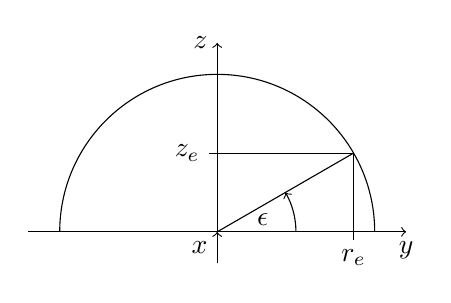
\begin{tikzpicture}[scale=2]
    \draw[->] (-1.2,0) -- (1.2,0) node[anchor=north] {$y$};
    \draw[->] (0,0) -- (0,1.2) node[anchor=east] {$z$};
    \draw[->] (0,-0.2) -- (0,0) node[anchor=north east] {$x$};
    \draw (0:1) arc (0:180:1);
    \draw (0:0) -- (30:1); 
    \draw[->] (0:0.5) arc (0:30:0.5);
    \node at (15:0.3) {$\epsilon$};
    \draw (-0.05,{sin(30)}) -- ({cos(30)},{sin(30)}) -- ({cos(30)},-0.05); 
    \node[anchor=east] at (-0.05,{sin(30)}) {$z_e$};
    \node[anchor=north] at ({cos(30)},-0.05) {$r_e$};
  \end{tikzpicture}
  \caption{Illustration of $z$-coordinate and radius of an elevated circle on
  a sphere}
  \label{fig:elevCirc}
\end{center}
\end{figure}

\noindent The respective screen coordinates are
\begin{align}
  \begin{pmatrix} x'(\varphi) \\ y'(\varphi) \\ z'(\varphi) \end{pmatrix}
  &= A \begin{pmatrix} x(\varphi) \\ y(\varphi) \\ z(\varphi) \end{pmatrix}
   = \begin{pmatrix}
       a_{xx} & a_{xy} & a_{xz} \\
       a_{yx} & a_{yy} & a_{yz} \\ 
       a_{zx} & a_{zy} & a_{zz} 
     \end{pmatrix}
     \begin{pmatrix} 
       r\cos\epsilon\cos\varphi \\ 
       r\cos\epsilon\sin\varphi \\ 
       r\sin\epsilon
     \end{pmatrix}
\\
  \notag
  &= \begin{pmatrix}
       a_{xx}\cdot r\cos\epsilon\cos\varphi + a_{xy}\cdot r\cos\epsilon\sin\varphi + a_{xz}\cdot r\sin\epsilon \\
       a_{yx}\cdot r\cos\epsilon\cos\varphi + a_{yy}\cdot r\cos\epsilon\sin\varphi + a_{yz}\cdot r\sin\epsilon \\
       a_{zx}\cdot r\cos\epsilon\cos\varphi + a_{zy}\cdot r\cos\epsilon\sin\varphi + a_{zz}\cdot r\sin\epsilon
     \end{pmatrix}\!\!.
\end{align}
Again, we determine the angle $\varphi_0$ where $z'(\varphi_0)=0$ by solving
\begin{align}
  0
  \stackrel{!}{=} z'(\varphi_0)
  &= a_{zx}\cdot r\cos\epsilon\cos\varphi_0 
   + a_{zy}\cdot r\cos\epsilon\sin\varphi_0 
   + a_{zz}\cdot r\sin\epsilon.
\end{align}
I frankly admit that I was too lazy to puzzle this out myself ;-\!) Matlab says
\begin{align}
  \tan\left(\frac{\varphi_0}{2}\right)
  &=\frac{a_{zy}\cos\epsilon \pm \sqrt{a_{zx}^2\cos^2\epsilon + a_{zy}^2\cos^2\epsilon - a_{zz}^2\sin^2\epsilon}}
         {a_{zx}\cos\epsilon - a_{zz}\sin\epsilon}
\\
  &=\frac{a_{zy} \pm \sqrt{a_{zx}^2 + a_{zy}^2 - a_{zz}^2\tan^2\epsilon}}
         {a_{zx} - a_{zz}\tan\epsilon},
\end{align}
where
\begin{equation}
  a_{zz}^2\sin^2\epsilon \ge (a_{zx}^2 + a_{zy}^2)\cos^2\epsilon
  \quad\leadsto\quad
  \tan^2\epsilon \ge \frac{a_{zx}^2 + a_{zy}^2}{a_{zz}^2}
\end{equation}
must hold. With the substitutions
\begin{align}
   u &= a_{zy}, \\ 
   v &= \sqrt{a_{zx}^2 + a_{zy}^2 - a_{zz}^2\tan^2\epsilon}\quad\text{and} \\ 
   w &= a_{zx} - a_{zz}\tan\epsilon 
\intertext{we get}
  \tan\left(\frac{\varphi_0}{2}\right)
  &=\frac{u \pm v}{w}
  \quad\leadsto\quad
  \varphi_0 = \begin{cases}
    2\atann(u+v,w)\\
    2\atann(u-v,w)  
  \end{cases}
\end{align}

\subsection{The Package Source Code}
\lstinputlisting[style=lstsLatex,linewidth=483pt]{tikz-3dplot-circleofsphere.sty}

\subsection{An Auxiliary Matlab Script}
\lstinputlisting[style=lstsMatlab,linewidth=483pt]{tikz_3dplot_circleofsphere.m}

\addcontentsline{toc}{section}{References}
\bibliographystyle{plain}
\bibliography{tikz-3dplot-circleofsphere}

\IfFileExists{_tester.tex}{
  \clearpage
  \LTXinputExample[style=lstsFrontPage]{_tester}
}{}

\end{document}

%% EOF